\section{Camera}

\begin{definition}[\textit{Camera}]
    A camera is an optical sensor that generates data using electric transducers. 
    It features an optical system designed to direct incoming light to its millions of photosensitive elements. 
    Modern cameras are typically capable of recording 30 to 60 frames per second.
\end{definition}
For simplicity, we will consider the optical system of a camera as a single lens with the following characteristics:
\begin{itemize}
    \item \textit{Spherical}: the lens is formed by the intersection of two spherical surfaces.
    \item \textit{Thin}: the distance between the centers of the two spheres is nearly equal to the sum of their radii.
    \item \textit{Small angles}: the light rays make only slight angles with respect to the optical axis.
\end{itemize}
These assumptions simplify the calculations involved in determining the path of a light ray as it passes through the lens. 
Specifically, the refraction of light at the boundary between two media is described by Snell's law:
\[\dfrac{\sin{\theta_2}}{\sin{\theta_1}}=\dfrac{n_1}{n_2}\]
Here: 
\begin{itemize}
    \item $\theta_1$ and $\theta_2$ are the angles between the normal at the surface and the direction of the light ray before and after crossing the boundary, respectively.
    \item $n_1$ and $n_2$ are the refractive indices of the two materials.
\end{itemize}
\begin{figure}[H]
    \centering
    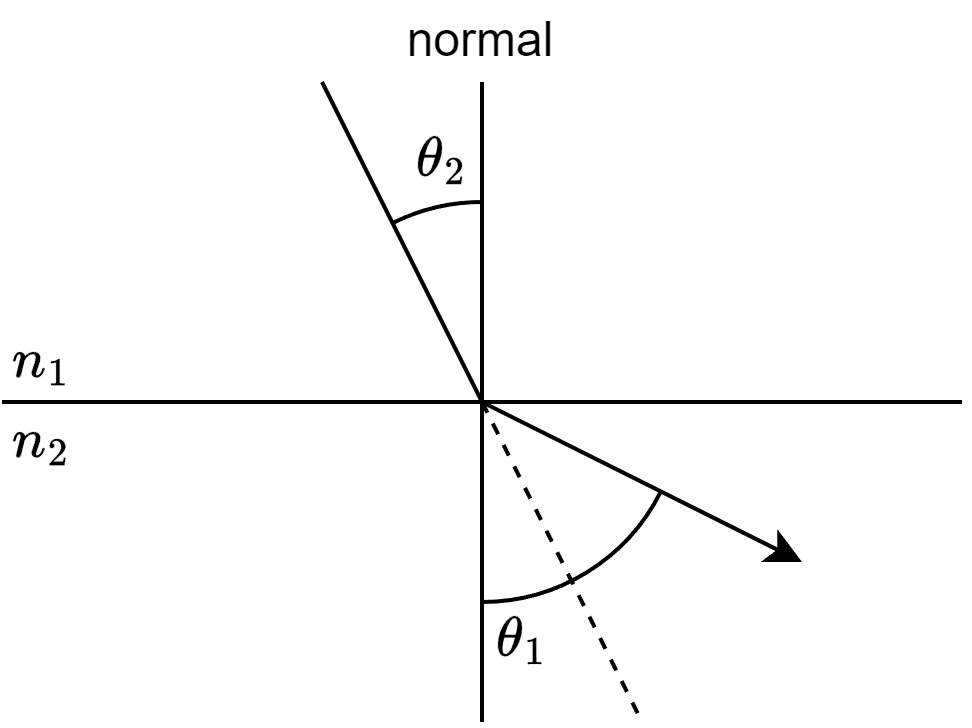
\includegraphics[width=0.4\linewidth]{images/refraction.png}
    \caption{Snell's law}
\end{figure}
\begin{definition}[\textit{Optical axis}]
    The optical axis is the straight line that connects the centers of the two spheres that form the lens.
\end{definition}
The angles of a ray passing through the centers of the spheres can be expressed as follows:
\[\alpha_1=\dfrac{y_1}{\rho_1} \qquad \alpha_2=-\dfrac{y_2}{\rho_2}\]
\begin{figure}[H]
    \centering
    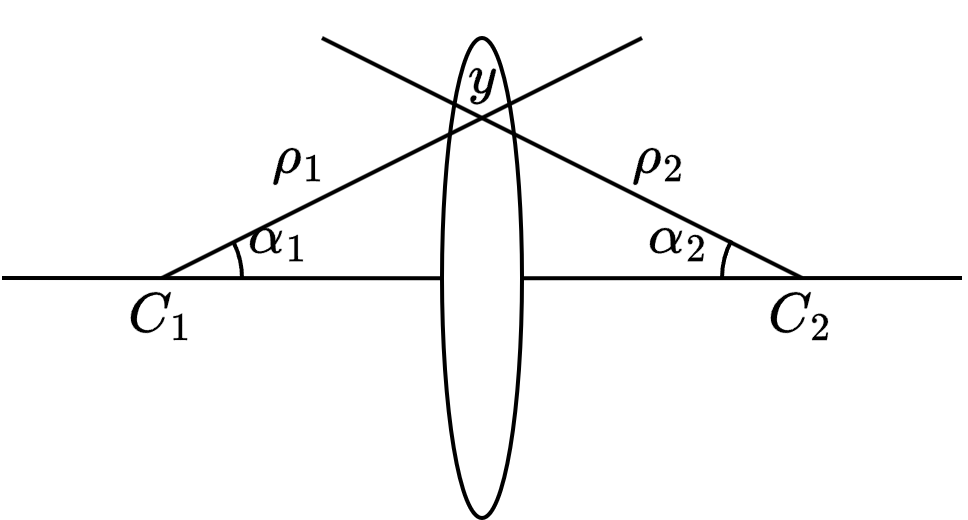
\includegraphics[width=0.4\linewidth]{images/y.png}
\end{figure}
In this context, with the simplified lens, it is reasonable to assume:
\[y_1=y_2=y\]